\documentclass{article}      % use "amsart" instead of "article" for AMSLaTeX format
\usepackage{graphicx}               % Use pdf, png, jpg, or eps§ with pdflatex; use eps in DVI mode
                                % TeX will automatically convert eps --> pdf in pdflatex   
\usepackage{caption}
\usepackage{subcaption}
\captionsetup{justification=raggedright,singlelinecheck=false}

\usepackage{amsmath}
\usepackage{amsthm}
\usepackage{amsfonts}
\usepackage{verbatim}
\usepackage{bm}
\usepackage{multicol}
\usepackage[switch]{lineno}
\usepackage{hyperref}

\usepackage{icml2025}


\newcommand{\cov}{\mathrm{cov}}

\usepackage{setspace}

\begin{document}
\twocolumn[
\icmltitle{Cumulant Generating Function Networks for Adaptation of Neural Network Statistics}

\begin{icmlauthorlist}
\icmlauthor{Luke Rast}{yyy}
\end{icmlauthorlist}

\icmlaffiliation{yyy}{Department of XXX, University of YYY, Location, Country}
\icmlcorrespondingauthor{Luke Rast}{first1.last1@xxx.edu}

\vskip 0.3in
]
\printAffiliationsAndNotice{}



\begin{abstract}
  Neural network performance suffers when input statistics differ between training and application data.
  The cumulant generating function provides access to classical methods for detecting and adapting to distributional changes.
  We learn cumulant generating functions that capture the statistics of internal layers in a trained neural network, and apply them to change detection and adaptation of the network.
  Specifically, we learn an input convex neural network representation of the cumulant generating function, and use saddlepoint approximation for change detection and exponential tilting for adaptation.
  Taking advantage of the neural network representation, we also learn a cumulant generating function representation of target-conditional distributions, allowing for application of Bayesian inference under label shift.
  We demonstrate these methods on simple examples.
\end{abstract}




\section{TLDR:}
Learning a neural network representation of the cumulant generating function provides access to simple methods for detecting and adapting to distribution shifts that can be applied to internal layers of neural networks.



\section{Overview}

In order to make this paper tight, we must show that the learned CGF solves multiple issues related to adaptation and distribution change: Change point detection via rate function, Adaptation through training on tilted distribution.
Additionally, we need to justify why the neural network representation is useful at all.
At the moment, this comes down to the fact that we can produce networks that capture the class-conditional distributions, thereby introducing parameterizations of the target distribution.

Honestly though, if we want any hope of this being useful to other people, we also need to demonstrate: 1. that CGF networks can actually be trained in high dimensions, and 2. that empirical CGFs work well to capture the statistic, even in high dimensions.

One critical thing that I need to demonstrate for this problem is the fidelity of the method for different tasks, and the behavior of the learned CGF under different conditions. 
This is probably the most important issue. Even more so than than coming up with different / novel methods for adjusting the networks. That said, a Bayesian adjustment based on the distribution is still appealing.


The core thing is: What are my actual claims?
\begin{itemize}
  \item Empirical CGFs can be leveraged for both domain adaptation and out-of-distribution detection
  \item ICNNs learn representations of the eCGF for both: marginal and class conditional cases, with class conditional being unique to the neural network representation
  \item Saddlepoint approximations perform well for change detection.
  \item Exponential tilting performs well for adaptation.
\end{itemize}





\section{Introduction and Background}


TO DO: Brief paragraphs on change detection and adaptation: Intro the change detection and adaptation problems.
Must dovetail into the need for a representation of the probability distribution.


Fitting the distribution of a random variable based on samples is often accomplished by learning a representation, parametric or non-parametric, of the probability density function.
Here, we instead fit probability distributions by learning a representation of the cumulant generating function.
We demonstrate that such representations are well suited to change detection and adaptation problems for neural networks.

The \textit{cumulant generating function} (CGF) of a random variable, $x$, is given by
\begin{equation}
  A(\theta) = \log \mathbb{E}_x[\exp(\theta^T x)]. \label{def:cgf}
\end{equation}
It is the logarithm of the moment generating function, and, when it exists, provides a unique representation of the distribution of $x$.
Importantly, the cumulant generating function is also guaranteed to be \textit{convex} \cite{barndorff2014information}.


One application of the CGF is constructing families of \textit{exponentially tilted} probability distributions \cite{morris_natural_1982,morris_unifying_2009}.
Starting from a baseline distribution $h(x)$, with cumulant generating function $A(\theta)$, exponential tilting produces the family
\begin{equation}
  p(x | \theta) = h(x) e^{\theta^T x - A(\theta)}. \label{def:exponential_tilt}
\end{equation}
This is a natural exponential family of distributions, each of which modifies the base measure $h(x)$ by concentrating the probability density along different directions to different extents.
The CGF gives the cumulant generating functions for every member of the tilted family
\begin{equation}
  A_\theta(\phi | \theta) = A(\theta + \phi) - A(\theta) \label{eq:CGF_family}
\end{equation}
Thus, the mean of any distribution in the family is given by the Jacobian of the CGF,
\begin{equation}
  \mu(\theta) = \nabla_\theta A(\theta) \label{eq:cgf_jacobian}
\end{equation}
while the Hessian gives the covariance matrix, and so forth \cite{barndorff2014information}.

Another application of the CGF is saddlepoint approximation \cite{daniels_saddlepoint_1954,barndorff-nielsen_edgeworth_1979}.
Given a distribution $h(x)$, with cumulant generating function $A(\theta)$, the saddlepoint approximates the distribution of sample means by
\begin{equation}
  p(\mu; n) \approx \left( \frac{n}{2\pi} \right)^{\frac{d}{2}} |V(\mu)|^{-1/2} \exp(-n I(\mu)). \label{def:mean_density}
\end{equation}
Where $\mu$ is the sample mean of $n$ samples in $d$ dimensions, $V(\mu)$ is covariance matrix (given by the Hessian of the CGF), and $I(\mu)$ is the rate function.
The \textit{rate function} is the Legendre transform of the cumulant generating function
\begin{equation}
  I(\mu) = \sup_{\theta}(\mu^T \theta  - A(\theta) ), \label{eq:legendre_transform}
\end{equation}
and corresponds to the rate function in large deviations theory, by Cramer's Theorem \cite{dembo2009large}.
The saddlepoint approximation becomes asymptotically tight as the number of datapoints increases \cite{iltis_sharp_1995,chaganty_multidimensional_1986}, but remains quite accurate at lower sample sizes \cite{davison_saddlepoint_1988,ronchetti_empirical_1994} as well.

In summary, given a cumulant generating function, we have access to two related functions, $A(\theta) \leftrightarrow I(\mu)$, the CGF and the rate function, related through Legendre duality.
Their arguments provide two related parameterizations $\theta \leftrightarrow \mu$ of the exponentially tilted family, corresponding to natural parameters $\theta$ and mean parameters, $\mu$.
Due to the duality, these are related by 
\begin{eqnarray}
  \mu = \nabla_\theta A(\theta) & \theta = \nabla_\mu I(\mu). \label{eq:duality_relations}
\end{eqnarray}
The function pair allows detection of changes in sample means, through the saddlepoint distribution~(\ref{def:mean_density}), and adaptation of the distribution that models the the sampling process, through exponential tilting~(\ref{def:exponential_tilt}).

We apply these dual functions to the twin problems of change detection and adaptation.
On one side of this duality, the rate function $I(\mu)$, gives the probability density over the mean of many samples.
We use this density to detect changes in the statistics of the world.
On the other side of the duality, the cumulant generating function $A(\theta)$ provides the basis for a family of modified versions of environmental statistics.
We use this family to adapt to changes in the statistics of the world.
We capture both functions using a learned representation of the cumulant generating function, the CGF network, together with the duality relations.

\subsection{Neural network applications}





We will use tilted distributions to adapt neural network activity.



In order to focus in on change detection and adaptation in the context of neural networks, we start with trained neural networks, and aim to track and respond to changes in the statistics of one of the hidden layers. 
We do this by learning a second neural network, which is trained to reproduce the empirical cumulant generating function for the activity of this hidden layer.
As an input convex neural network \cite{amos_input_2017} this representation of the CGF is guaranteed to be convex and is easily differentiable, giving access to both the CGF and the rate function.
We take advantage of the rate function...




Explore direct representation of the cumulant generating function 

Non-parameteric CGF, with parameterized 



\section{Related work}


Previous works on adaptation more generally

Previous works on exponential tilting: finance, ML, adaptation 


What is the connection to previous free energy based approaches?


Averaging enough data points will allow us to determine whether the network activity follows the same statistics as the training data using either element-wise test on each dimension, as in \cite{rabanser_failing_2019} or a joint test on the all dimensions simultaneously.


Change detection, which aims to detect changes in the statistics of the environment is a significantly easier task than anomaly detection, which aims to detect individual points that are not from the training set distribution.


\subsection{Adaptation by importance weighting}





\subsection{Convex optimization layers and convex networks}




\subsection{Connection to VAEs}

Our approach is related to variational autoencoders (VAEs) \cite{kingma_auto-encoding_2013}, which learn to perform approximate inference under specified noise and latent variable distributions. 
Our model instead performs exact inference with a learned noise distribution and its conjugate, at the cost of decreased flexibility in possible conditional distributions.
Concretely, we use learned neural network features $T(x)$ as sufficient statistics and learn the cumulant generating function $A(\theta)$ that captures the base measure on these features.
This specifies an exponential family, the set of exponentially tilted distributions, whose parameters determined through exact inference.
Thus, while VAEs correspond to an \textit{outer approximation} using approximate inference, our approach gives an \textit{inner approximation} of inference by using family of distributions for whom inference is always exact.
This process can produce any exponential family.
In this work, we learn the sufficient statistics and cumulant generating function in turn, but extension to learning these simultaneously is an important future direction.





\section{Results}

We use a learned cumulant generating function to track the internal statistics of a neural network, and to compare these internal statistics in novel environments.
Assume that we have a neural network, $\mathcal{N}_0$, that is trained for a classification task, mapping inputs, $x$, to target labels, $y$.
Given the trained network $\mathcal{N}_0$, we choose one hidden layer of the network, which we denote $T=T(x)$ to be our feature vector, and train a second neural network, which we call the \textit{CGF network} $A(\theta)$, to capture the statistic of $T(x)$ across inputs by reproducing its cumulant generating function. 
Combining $T(x)$ and $A(\theta)$ using exponential tilting (\ref{def:exponential_tilt}) gives an exponential family of distributions over $x$, with sufficient statistics $T(x)$ that are the features learned by $\mathcal{N}_0$.

\subsection{CGF networks}
We parameterize the CGF network using an input convex neural network \cite{amos_input_2017,hoedt_principled_2023}, which ensures that the learned CGF is convex, and that its derivatives can be evaluated by auto-differentiation.
We train the CGF network to reproduce the values of the empirical cumulant generating function (eCGF)
\begin{equation}
  \hat A(\theta) = \log \left( \frac{1}{N}\sum_{i} \exp(\theta^T T_i) \right), \label{def:empirical_CGF}
\end{equation}
which uses the empirical mean to evaluate the expectation in the CGF. 
This expression has previously been used as a CGF estimator for $n$ dimensional data \cite{davison_saddlepoint_1988,ronchetti_empirical_1994} in the context of saddlepoint approximation.

We train the CGF network by randomly sampling a variety of $\theta$ input values and training the network to produce the value of $\hat A(\theta)$ from expression (\ref{def:empirical_CGF}).
As show in Figure~\ref{fig:1a_CGF_Normal} for data with unit variance, the empirical CGF accurately captures the ground truth CGF at $\theta$ values that are close to zero.
However, it begins to diverge as $\theta$ moves farther from the origin, with limiting behavior that is linear rather than quadratic. 
The CGF network perfectly mimics the behavior of the eCGF.
However, evaluating the corresponding probability density (as described below), we recover a quite accurate approximation of ground truth, Figure~\ref{fig:1a_CGF_Normal}.
This shows that it is most important to capture the values of the empirical CGF at inputs close to the origin.
Because of this, we always sample training values of $\theta$ that are concentrated around the origin (regardless of the dimensionality).
We also preprocess data coming into the CGF network to have zero mean and unit variance, across all dimensions. 
See Section~\ref{sec:network_architecture} for full details of our CGF network, training, and preprocessing.

\begin{figure}[tb]
  \centering
  \begin{subfigure}[t]{0.5\textwidth}
    \centering
    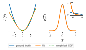
\includegraphics[]{figures/figure1a.pdf}
    \caption{Univariate standard normal distribution, 5k samples. Left: CGF, Right: pdf, Inset: pdf zoomed around $x=4.9$}
    \label{fig:1a_CGF_Normal}
  \end{subfigure}
  \begin{subfigure}[t]{0.5\textwidth}
    \centering
    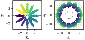
\includegraphics[]{figures/figure1b.pdf}
    \caption{Class-conditional distribution, 4k samples. Left: scatterplot of the data, colored by target, Right: scatter plot of parameter samples $\theta(y) + \phi$ , colored by conditional eCGF value, contours show the conditional CGF network fits}
    \label{fig:1b_conditional_CGF}
  \end{subfigure}

  \caption{Learned Cumulant generating functions of simple distributions. (a): CGF network fits to univariate normal distribution (b): conditional CGF network fits to bivariate, target conditional normal distribution}
  \label{fig:1_CGF}
\end{figure}


Given the CGF network representation of $A(\theta)$, we can also evaluate the dual rate function $I(\mu)$ (Eq.~\ref{eq:legendre_transform}) and transform $\theta \leftrightarrow \mu$ between equivalent values of the natural and moment parameters.
Following equation~(\ref{eq:duality_relations}), we compute the mean parameters $\mu(\theta)$ using the Jacobian of the neural network. 
Evaluation of $I(\mu)$ and $\theta(\mu)$ both come down to evaluating the Legendre transform (Eq.~\ref{eq:legendre_transform}), which we do by directly solving the optimization problem using gradient descent in $\theta$.
The resulting optimal input gives $\theta(\mu)$, while the optimal value is $I(\mu)$.
Note that more sophisticated optimization approaches are also available.

We use the rate function $I(\mu)$ and the determinant of the Hessian, ${V(\mu) = \bm{H}[A](\theta(\mu))}$, to compute the saddlepoint approximation of the probability density, Eq.~(\ref{def:mean_density}).
Figure~\ref{fig:1a_CGF_Normal} shows this approximate probability density for univariate Gaussian data.
The approximation is quite good, but shows a characteristic deviations in the tails, highlighted in the inset:
the approximate pdf falls sharply to zero beyond a cut-off point. 
This is the result of the fact that the empirical CGF becomes linear at large values, meaning that the Legendre transform diverges to infinity for $\mu$ values exceeding the maximum (or minimum) slope.
The linearity of the eCGF, in turn, can be understood from Equation~(\ref{def:empirical_CGF}): as $\theta$ gets large, the sum is increasingly dominated by only the term with the largest $T_i$ value.
The result is that the limiting slopes, and therefore the cut-off values of the approximate density, are dominated by the extreme values in the training data: the approximate probability decays exponentially outside the range of observed datapoints.



\subsection{Conditional CGF networks}

Rather than learning a CGF network representation of the distribution of $T(x)$ as a whole, we can alternatively learn a \textit{conditional CGF network} representation that captures the target-conditional distributions, $p(T|y)$.
In order to do this, we assume a target-to-parameter mapping, $\theta(y)$, which we take as given, and fit $A(\theta)$ to ensure that exponentially tilted distributions
\begin{equation}
  p(T|y) = h(T) \exp(\theta(y)^T T - A(\theta(y))) \label{eq:class_conditional}
\end{equation}
capture the observed conditional distributions.
In other words, we impose a requirement on the learned $A(\theta)$ that exponential tilting in each of the specific directions $\theta(y_i)$ should produce the conditional distribution $p(T|y_i)$.

We do this using Equation (\ref{eq:CGF_family}) for the cumulant generating function of tilted distributions.
For every target class $y_i$, the tilted CGF $A_{\theta(y_i)}(\phi | \theta(y_i))$ should match the CGF of the data with label $y_i$.
In order accomplish this, we sample a variety of $\phi$ values for each target class and evaluate the \textit{class-conditional} empirical CGF $\hat A_{y_i}(\phi)$ using only data with label $y_i$.
This produces the dataset $\{\phi_{i}, \theta(y_i), \hat A_{y_i}(\phi_i)\}$.
We then train our conditional CGF network $A(\theta)$ to minimize the distance between ${A(\theta(y_i) + \phi_i ) - A(\theta(y_i))}$ and $\hat A_{y_i}(\phi_i)$.

We show an example of this approach Figure~\ref{fig:1b_conditional_CGF}.
In this example, the target-to-parameter mapping $\theta(y)$ is set so that $\theta(y_i)$ points in the same direction as the mean of the data conditional on $y_i$, and has magnitude 12.
Looking at the right side of Figure~\ref{fig:1b_conditional_CGF}, there are two things to note about this parameter embedding.
First, adjusting the magnitude of the parameter embedding will change how much overlap there is between the point clouds, and therefore how easily the conditional CGF can be fit. 
Second, the point clouds are arranged in a way that produces a convex function: the color gradients all align outward from the origin. 
This would not be case if the locations of the clouds were shuffled. 
This is an important minimum requirement for any parameter embedding.
The orientation of the color gradient in the conditional eCGFs of Figure~\ref{fig:1b_conditional_CGF} correspond to their Jacobian, and therefore to the class conditional means.
Through-out this work we will use the same parameter embedding: we set the parameters to be aligned with the class-conditional means, but with a large, fixed magnitude of 12.


\subsection{Change point detection}
Given a trained cumulant generating function network, which captures the statistics of the internal activity data that it was trained on, we first want to detect whether newly observed data follows the same statistics.
The CGF plugs easily into methods for change detection.

\textbf{Score test:} \cite{cox1979theoretical} 
Given the family of exponentially tilted distributions (\ref{def:exponential_tilt}), we test whether observed data is consistent with $\theta = 0$, which corresponds to the base distribution that $A(\theta)$ was trained on.
The score test does this in the large data limit, by testing whether the data average is consistent with a multivariate normal distribution with mean $\frac{\partial}{\partial \theta_i} A(\theta)$ and covariance $\frac{1}{n}\frac{\partial^2}{\partial \theta_i \partial \theta_j} A(\theta)$, using a Chi-square distribution.
This is equivalent to approximating the activity distribution with a multivariate normal distribution, and so can be viewed as a negative control for our method. 

\textbf{Rate function tests:} Refining the idea of the score test, we can instead use the asymptotic mean probability density (\ref{def:mean_density}), which (as a large deviations principle) we anticipate to be more accurate at moderate sample sizes than the normal assumption.
Because the rate function $I(\mu)$ is increasing, we use level curves of the rate function to delineate a significance region, by finding a radius $r_\alpha$ such that ${p(I(\mu) \le r_\alpha) = 1 - \alpha}$.
Alternatively, we can include the determinant term in the saddlepoint approximation by using level curves of log-likelihood to delineate significance regions.
Either way the radius of such a region can be determined by binary search, together with importance sampling to approximate the probability of falling in this region.

We show the performance of each of these change detection methods 

\subsection{Adaptation through exponential tilting}
Once we detect a significant change in the internal statistic of our neural network, we then want to correct our model to account for that change.
We can use the learned CGF network to correct for changes in input statistics in several different ways.

\textbf{Fine-tuning:} Following the approach of \cite{maity_understanding_2023}, we model the new feature distribution as an exponentially tilted version (\ref{def:exponential_tilt}) of the training distribution  under some values $\hat \theta$ of the parameters.
We determine $\hat \theta$ based on the mean value of the activity that we observe ${\hat \theta = \theta(\hat \mu) = \theta(\frac{1}{n} \sum_i T_i)}$, using the CGF network to compute $\theta(\mu)$ as in (Eq.~\ref{eq:duality_relations}).
Given parameters $\hat \theta$, the exponential tilt equation gives importance weights ${\exp(\hat \theta^T T - A(\hat \theta))}$, which we use to fine-tune the network by training on the original training data, with each point weighted by its importance value under the new feature distribution.
In order to avoid having the retrain the CGF network, we freeze the weights of the original network $\mathcal{N}_0$ below our hidden layer of interest, and fine-tune the top half of the network.


\textbf{Inference:}
Given a class-conditional CGF representation, we replace the top half of our original network $\mathcal{N}_0$ with Bayesian inference.
Assume that we have a prior $p(y)$ over labels and a conditional CGF representation of the likelihood $p(T|y)$.
Then, the log-posterior over labels is ${\log p(y|T) = \log p(y) + \theta(y)^T T - A(\theta(y)) + C_0(T)}$ where $C_0$ accumulates terms that do not depend on $y$.
Softmax gives a normalized posterior.
The inference approach is useful for \textit{label shift} [REF], which assumes that the probability labels $p(y)$ changes between environments, while the conditional distribution $p(x|y)$ (and therefore $p(T(x)|y)$) remains unchanged.
In this case, adaptation to the new environment requires only a change in $p(y)$, which we fit by regressing observed means against the parameter dependent means: ???.



\subsection{Example: MNIST classifier}

We apply these techniques to the simple case of a multilayer percepetron with one hidden layer of width 28, trained for classification of MNIST dataset.
Based on the activity of the hidden layer across all training points in the MNIST dataset, we train a CGF network and a conditional CGF network, which attain validation mean squared error of $\sim 0.04$ and $\sim 0.06$ respectively, indicating that they are, at minimum, fitting the eCGF reasonably well in the sampled regions.

\begin{figure}[tbh]
  \centering
  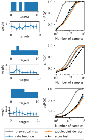
\includegraphics[]{figures/figure2.pdf}
  \caption{Change Detection: area under the ROC curves for a variety of label distribution with a variety of different performances.}
  \label{fig:2_change_detection}
\end{figure}

First, we evaluate the performance of the CGF network model at change detection, when the frequencies of the targets label are modified.
As shown in Figure~\ref{fig:2_change_detection}, we see a variety of change detection performances for 



In , we show a variety of detection behaviors 


the area under the ROC curve for detection of changes from uniform label distribution to alternative


There are several things that are worth noticing from the plots
little difference between using rate function and full saddlepoint density










\begin{figure}[tb]
  \centering
  \begin{subfigure}[t]{\textwidth}
    \centering
    %\includegraphics[]{}
    \caption{}
    \label{fig:3a_adaptation_example}
  \end{subfigure}

  \caption{Applications to network adaptation }
  \label{fig:3_adaptation_example}
\end{figure}




\newpage
\subsection{RAW}

\noindent \textbf{Questions and other things to write about:}
\begin{itemize}
  \item How many training samples do I need as a function of dimensionality to learn the CGF? This could be an argument for using the dimensionality reduction by the neural network features.
  \item How well does the empirical CGF work as a normalizer?
  \item Evaluation of how well the learned functions capture the duality relationships.
  \item How well does conditional work for different $\theta(y)$?
  \item How does the accuracy of the marginal for a given conditional depend on the assumptions about $\theta(y)$?
  \item Contribution of the determinant term to the saddlepoint approximation.
  \item How to update CGF parameters after finetuning to continue to use as a change detector
  \item Conditional CGF approach for change detection. 
\end{itemize}






\newpage




\section{Conclusion}

In this work, we have demonstrated the 


Future direction: learning $T(x)$ together with sufficient statistics.


and the same process can be extended to produce any exponential family, by combining a set of statistics of the data, $T(x)$, and a base distribution of these statistics.
This is the path that we pursue in this paper: we will learn exponential families by learning both $T(x)$ and $M(\theta)$ and use these learned families to perform inference.



One sentence relationship to VAE


Future directions:

Extension to multiple CGF networks, one for each layer of the network 
Learning the parameter curves in conditional networks


In this work, we assume a specified target-to-parameter mapping, $\theta(y)$.
Learning such a mapping together with the CGF is an important future direction.


We demonstrated this method for the special case of label shift, however the approach is not limited to this case.
In particular, rate-function change detection and fine-tuning on exponentially tilted data are applicable to arbitrary distributional shifts.



\section{Models and methods}

Code for these models is available on github: \texttt{placeholder}

\subsection{CGF Network} \label{sec:network_architecture}

The CGF network is an input convex neural network \cite{amos_input_2017}, with convex non-linearities and positive weights after the first layer.
We use a multi-layer perceptron with no skip connections, but with positive weight matrices initialized as in \cite{hoedt_principled_2023}, and guaranteed to be positive by a ReLU applied to the weights.
For non-linearities, we use a leaky version of a softplus, given by $sp_{\textrm{leaky}}(x) = \alpha x + (1 - \alpha) sp(x) + c_0$ where $sp(x)$ is a softplus function, $\alpha$ sets the leak slope for negative values, and $c_0$ sets the intercept. 
These values are set to $\alpha =0.05$ and $c_0 = -0.693$, which sets the intercept to be the origin.
We choose the leaky softplus because it is convex (as required) and continuously differentiable, giving smooth Jacobians and Hessians, while retaining the benefits of leaky ReLUs in preventing dead units.
Additionally, it allows negative values to pass through the network, which is particularly important in the ICNN case, where the network weights are constrained to be positive.
We use three hidden layers, with widths of 200.

We generate the values of $\theta$ for the training set by sampling vectors with uniform orientations and lengths that are distributed according to a $\chi_1$ distribution, analogous to a univariate normal distribution.
The scale of the length distribution is set to $\sqrt{5}$.
This sampling method ensures that our samples are concentrated around the origin regardless of dimensionality, avoiding the well-known issue with high-dimensional multivariate normal distributions.
We find that about $10^6$ sample $\theta$ values are sufficient to achieve good fits to the eCGF.


We preprocess the activity data used as input to our CGF networks by removing the mean, and dividing by the variance across all dimension.
That is to say, we evaluate the mean $m = \frac{1}{n} \sum_i T_i$ and the variance ${v = \frac{1}{n}\sum_{ij} \left(T_{ij} - \frac{1}{n}\sum_{ij} T_{ij} \right)^2}$ of the training data, and transform all data $D$ to
\begin{equation}
  D_{\textrm{post}} = (D - m) /\sqrt{v}
\end{equation}
Note that $v$ is the \textit{scalar variance} across all dimensions of the data.
We use this method to produce centralized data without changing the structure or the relative importance of any dimension.

We perform dual optimization by gradient descent. We observed that different optimization hyper-parameters are better for different contexts.
Adam with small learning rate performs better in high dimensions, while SGD with momentum and large learning rate is preferable in lower dimensions.
This could be optimized by a hyper-parameter screen, but we stick to hand-tuning for the results in this paper.
Note that new data can be generated for dual evaluation, with the Jacobian of the forward model providing a means of evaluating the quality of the outputs.




\subsection{Model MNIST networks} \label{sec:model_network_details}

The MNIST network is a multilayer perceptron with one hidden layer and layer widths (784, 28, 10).
We train on the MNIST training data from the library \texttt{torchvision} with an 95\%-5\% train-validation split and early stopping.

In order to achieve exactly balanced target-class frequencies during training,  we upsample underrepresented classes in the dataset, and ensure that training and validation splits are perfectly balanced. 
This model achieves ???\% test accuracy.








\section*{Acknowledgements}

\texttt{Placeholder}

\section*{Impact Statement}
This paper presents work whose goal is to advance the field of 
Machine Learning. There are many potential societal consequences 
of our work, none which we feel must be specifically highlighted here.


\section{OLD MATERIAL: Brainstorming}

Reformulate

Leveraging duality 

Leveraging learned CGF

Learn the cumulant generating function, and leverage it's properties, in particular duality to the rate function.

\begin{itemize}
  \item Learned CGF fits distributional families and it fits them well.
  \item Learned CGF facilitates change point detection via: multiple test possibilities
  \item Learned CGF facilitates adaptation via: multiple adaptation possibilities
\end{itemize}

\section{Questions still unanswered}
\begin{itemize}
  \item What size of networks do we need to fit higher dimensional data?
\end{itemize}


Equivalently, the slope of the eCGF is determined by the empirical cumulative distribution function, and therefore becomes constant beyond a certain point.

\bibliography{main.bib}
\bibliographystyle{icml2025}

\end{document}